% ============================================================
% 第1章 化学反应的热效应（对应课件：选必一1.1 反应热、1.2 反应热的计算）
% ============================================================
\chapter{化学反应的热效应}

\begin{daoxue}
\textbf{知识主线：}反应热是什么（体系与环境、焓变）$\to$ 为什么有反应热（键能、物质能量）$\to$ 怎样测（中和反应反应热）$\to$ 怎样表示（热化学方程式、燃烧热）$\to$ 怎样算（盖斯定律等六种方法）。

\textbf{高考考情：}广东卷第19题（原理综合）几乎每年第一或第二小问考“盖斯定律求 $\Delta H$”（2024第19题(1)②、2025第19题(3)①、2026第19题(2)），约2分，必须稳拿；选择题常以“能量—反应进程图”考查放热吸热、活化能与催化剂（2024第15题、2026第15题）。

\textbf{学习目标：}①能从宏观（物质能量）和微观（化学键）两个角度解释反应热；②会规范书写热化学方程式并判断正误；③能熟练用盖斯定律、键能、燃烧热等计算 $\Delta H$，并会比较 $\Delta H$ 大小。
\end{daoxue}

\section{反应热与焓变}

\subsection{体系、环境与反应热}
研究化学反应的热效应，首先要划定研究对象。被研究的物质系统叫\textbf{体系}（如试管中的盐酸、NaOH溶液及发生的反应），与体系相互影响的其他部分叫\textbf{环境}（如试管、空气）。热量总是在体系和环境之间传递。

\begin{tuozhan}[三种热力学体系]
按体系与环境之间有无物质和能量交换，可分为：\textbf{敞开体系}（既有物质交换又有能量交换，如敞口烧杯中的反应）、\textbf{封闭体系}（只有能量交换、没有物质交换，如密闭容器中的反应）、\textbf{孤立体系}（既无物质交换也无能量交换，如理想的绝热密闭容器）。量热计的设计思路，就是尽量使反应体系接近“与外界无热交换”的状态，从而准确测出温度变化。
\end{tuozhan}

\begin{gainian}[反应热]
在\textbf{等温}条件下（反应前后体系温度相同），化学反应体系向环境释放或从环境吸收的热量，称为化学反应的热效应，简称\textbf{反应热}。
\end{gainian}

为什么强调“等温”？反应放出的热量会先使体系温度升高，只有让体系恢复到反应前的温度，传给环境的热量才完全由“化学变化”本身决定，否则一部分能量还“存”在体系的升温里。量热计测得的温度变化，正是用来反推这部分热量的。

\subsection{焓与焓变}
化学反应之所以有热效应，是因为反应前后体系的\textbf{内能}（$U$，体系内物质各种能量的总和）发生了变化。生产和科研中的反应大多在\textbf{等压}（敞口，压强等于大气压）下进行，为方便描述，引入与内能有关的物理量——\textbf{焓}（$H$）。

\begin{gainian}[焓变]
中学阶段规定：等压条件下进行的化学反应，其反应热等于反应的焓变，用 $\Delta H$ 表示，单位 kJ·mol$^{-1}$。
\[\Delta H=H(\text{生成物})-H(\text{反应物})\]
放热反应：体系能量降低，$\Delta H<0$；\quad 吸热反应：体系能量升高，$\Delta H>0$。
\end{gainian}

注意 $\Delta H$ 的正负号是“站在体系的立场”说的：体系放出热量，自身焓减少，故为负。“$\Delta H=-92.4$ kJ·mol$^{-1}$”中的“$-$”表示放热，不是“数值小”。

\subsection{从宏观角度认识：物质的能量}
\begin{center}
\begin{tikzpicture}[scale=0.72]
\begin{scope}
\draw[-Stealth] (0,0)--(4.4,0) node[below left]{\small 反应进程};
\draw[-Stealth] (0,0)--(0,3.3) node[left]{\small 焓 $H$};
\draw[thick] (0.4,2.4)--(1.6,2.4) node[midway,above]{\small 反应物};
\draw[thick] (2.6,0.8)--(3.8,0.8) node[midway,above]{\small 生成物};
\draw[-Stealth,warnred,thick] (2.2,2.4)--(2.2,0.8) node[midway,left]{\small$\Delta H<0$};
\node at (2.1,-1.0) {\small 放热反应};
\end{scope}
\begin{scope}[xshift=6.5cm]
\draw[-Stealth] (0,0)--(4.4,0) node[below left]{\small 反应进程};
\draw[-Stealth] (0,0)--(0,3.3) node[left]{\small 焓 $H$};
\draw[thick] (0.4,0.8)--(1.6,0.8) node[midway,above]{\small 反应物};
\draw[thick] (2.6,2.4)--(3.8,2.4) node[midway,above]{\small 生成物};
\draw[-Stealth,mainblue,thick] (2.2,0.8)--(2.2,2.4) node[midway,left]{\small$\Delta H>0$};
\node at (2.1,-1.0) {\small 吸热反应};
\end{scope}
\end{tikzpicture}
\end{center}

\begin{center}
\small
\begin{tabularx}{\linewidth}{>{\centering\arraybackslash}p{1.6cm}X}
\toprule
类型 & 常见实例 \\
\midrule
放热反应 & 燃烧；酸碱中和；活泼金属与水或酸；大多数化合反应；铝热反应；物质的缓慢氧化；\ce{2H2O2 = 2H2O + O2 ^}（分解但放热） \\
吸热反应 & 大多数分解反应；\ce{Ba(OH)2*8H2O} 与 \ce{NH4Cl} 的反应；\ce{C + H2O(g) ->[\text{高温}] CO + H2}；\ce{C + CO2 ->[\text{高温}] 2CO}（化合但吸热） \\
\bottomrule
\end{tabularx}
\end{center}

\begin{yicuo}
\begin{enumerate}
\item 反应吸热还是放热，只由反应物和生成物的能量相对高低决定，\textbf{与反应条件无关}。需要加热的反应不一定吸热（如木炭燃烧需点燃）；不需加热的反应也可能吸热（如 \ce{Ba(OH)2*8H2O} 与 \ce{NH4Cl} 常温搅拌即可反应）。“停止加热后仍能持续进行”的反应一般是放热反应。
\item “吸热反应”“放热反应”专指\textbf{化学反应}。浓硫酸稀释、NaOH 固体溶解放热，\ce{NH4NO3} 溶解吸热，水的汽化吸热，都是物理过程，不能叫“放热反应”或“吸热反应”。
\end{enumerate}
\end{yicuo}

\subsection{从微观角度认识：化学键的断裂与形成}
化学反应的本质是旧化学键断裂、新化学键形成。\textbf{断键要吸收能量，成键会释放能量}——两个原子靠近成键后能量降低才稳定，要把它们拉开就必须从外界补充同样多的能量。

\begin{gainian}[键能]
25 ℃、101 kPa 下，断开 1 mol 气态分子 AB(g) 中的共价键，使其生成气态原子 A(g) 和 B(g) 所吸收的能量。键能越大，化学键越牢固，含该键的分子越稳定。
\end{gainian}

以 \ce{H2(g) + Cl2(g) = 2HCl(g)} 为例（键能：H—H 436、Cl—Cl 243、H—Cl 431，单位 kJ·mol$^{-1}$）：断开 1 mol H—H 和 1 mol Cl—Cl 共吸收 $436+243=679$ kJ；形成 2 mol H—Cl 共放出 $2\times431=862$ kJ。放出多于吸收，净放热 183 kJ，即 $\Delta H\approx-183$ kJ·mol$^{-1}$，与实验值 $-184.6$ kJ·mol$^{-1}$ 很接近。这说明：\textbf{化学键断裂和形成时的能量变化，是化学反应中能量变化的主要原因}。

\begin{benzhi}[为什么 $\Delta H=\sum E(\text{反应物键能})-\sum E(\text{生成物键能})$]
设想反应分两步走：第一步把反应物的键全部拆成气态原子，吸热 $\sum E_\text{反}$（焓增加）；第二步原子重新组合成生成物，放热 $\sum E_\text{生}$（焓减少）。由于焓变只与始终态有关（见1.5节），$\Delta H=(+\sum E_\text{反})+(-\sum E_\text{生})$。所以“\textbf{键能算焓变：反应物减生成物}”，而“\textbf{物质能量算焓变：生成物减反应物}”，两者顺序恰好相反，原因是\textbf{键能越大，物质本身的能量反而越低}。
\end{benzhi}

用键能计算时，关键是数清 1 mol 物质中含多少摩尔化学键，特别是空间网状或特殊结构的物质：

\begin{center}
\small
\begin{tabular}{cccccccc}
\toprule
物质 & \ce{P4}（白磷） & 晶体硅 & \ce{SiO2} & 金刚石 & 石墨 & \ce{S8} & \ce{CO2} \\
\midrule
1 mol 中键的物质的量 & 6 mol P—P & 2 mol Si—Si & 4 mol Si—O & 2 mol C—C & 1.5 mol C—C & 8 mol S—S & 2 mol C=O \\
\bottomrule
\end{tabular}
\end{center}

\begin{liti}[键能计算]
\ce{SF6} 是一种优良的绝缘气体，分子中只存在 S—F 键。已知：1 mol S(s) 转化为气态硫原子吸收能量 280 kJ，断裂 1 mol F—F、1 mol S—F 分别需吸收能量 160 kJ、330 kJ。则 \ce{S(s) + 3F2(g) = SF6(g)} 的 $\Delta H$ 为
\xx{$-1780$ kJ·mol$^{-1}$}{$-1220$ kJ·mol$^{-1}$}{$-450$ kJ·mol$^{-1}$}{$+430$ kJ·mol$^{-1}$}
\tcblower
\silu “吸收的减去放出的”：使反应物变成气态原子所吸收的能量 $-$ 由气态原子形成生成物所放出的能量。\\
\jie 吸收：$280+3\times160=760$ kJ；放出：1 个 \ce{SF6} 含 6 个 S—F 键，$6\times330=1980$ kJ。$\Delta H=760-1980=-1220$ kJ·mol$^{-1}$。\daan B\\
\xianjing S(s) 变为气态 S 原子既要克服分子间作用力，又要断开 \ce{S8} 环中的 S—S 键，题目已直接给出“S(s)$\to$S(g)”的总能量，照用即可，不要再另算 S—S 键；不要漏乘 6。
\end{liti}

\section{中和反应反应热及其测定}

\begin{gainian}[中和反应反应热]
在稀溶液中，强酸和强碱发生中和反应生成 1 mol \ce{H2O(l)} 时所放出的热量。25 ℃、101 kPa 下：
\[\ce{H+(aq) + OH-(aq) = H2O(l)}\qquad \Delta H=-57.3\ \mathrm{kJ\cdot mol^{-1}}\]
（旧教材称“中和热”，新教材称“中和反应反应热”，含义相同。）
\end{gainian}

\textbf{实验原理：}用简易量热计（内筒、隔热层、外壳、杯盖、温度计、玻璃搅拌器）测出反应前后溶液的温度差，再由 $Q=cm\Delta t$ 求热量。

\textbf{实验步骤与数据处理：}用量筒量取 50 mL 0.50 mol·L$^{-1}$ 盐酸倒入内筒，测温；洗净并擦干温度计，再量取 50 mL 0.55 mol·L$^{-1}$ NaOH 溶液测温（取两者平均值为 $t_1$）；将 NaOH 溶液\textbf{一次迅速}倒入内筒，盖好杯盖，匀速搅拌，记录\textbf{最高温度} $t_2$；重复实验 2 次，取温差平均值。近似认为溶液密度为 1 g·mL$^{-1}$、比热容 $c=4.18$ J·g$^{-1}$·℃$^{-1}$：
\[Q=(50+50)\,\mathrm{g}\times4.18\times10^{-3}\,\mathrm{kJ\cdot g^{-1}\cdot ℃^{-1}}\times(t_2-t_1)=0.418(t_2-t_1)\ \mathrm{kJ}\]
生成 \ce{H2O} 为 0.025 mol，故 $\Delta H=-\dfrac{0.418(t_2-t_1)}{0.025}\ \mathrm{kJ\cdot mol^{-1}}$。

\begin{benzhi}[实验中的五个“为什么”]
\begin{enumerate}
\item \textbf{为何 NaOH 稍过量（0.55 vs 0.50）？}保证盐酸完全被中和，生成水的量由盐酸确定为 0.025 mol。
\item \textbf{为何要一次迅速倒入？}分多次或缓慢倒入，热量在操作中散失，$\Delta t$ 偏小。
\item \textbf{为何不能用铜（金属）搅拌器？}金属导热快，热量损失大。
\item \textbf{为何测完酸要洗净温度计再测碱？}否则残留的酸与碱在温度计上反应放热，使测得的碱初温偏高，$\Delta t$ 偏小。
\item \textbf{改用 100 mL 0.50 mol·L$^{-1}$ 盐酸与 100 mL 0.55 mol·L$^{-1}$ NaOH，结果会翻倍吗？}放出的总热量翻倍，但中和反应反应热是“生成 1 mol \ce{H2O}”的热量，数值基本不变。
\end{enumerate}
\end{benzhi}

\begin{center}
\small
\begin{tabularx}{\linewidth}{Xc}
\toprule
误差来源（与理论值 57.3 kJ·mol$^{-1}$ 比较测得的放热数值） & 结果 \\
\midrule
装置保温、隔热差；分多次加入碱液；用铜质搅拌器；温度计未洗直接测碱温 & 偏小 \\
用弱酸（如 \ce{CH3COOH}）或弱碱（如氨水）代替：弱电解质电离要吸热 & 偏小 \\
用浓硫酸或 NaOH 固体代替稀溶液：溶解（稀释）放热 & 偏大 \\
用稀硫酸与 \ce{Ba(OH)2} 溶液：生成 \ce{BaSO4} 沉淀也放热 & 偏大 \\
量取盐酸时仰视读数：实际 HCl 多于 0.025 mol，生成水多，但仍按 0.025 mol 计算 & 偏大 \\
\bottomrule
\end{tabularx}
\end{center}

\begin{liti}[误差分析]
某同学测得稀盐酸与稀 NaOH 溶液反应生成 1 mol \ce{H2O(l)} 放出热量 52.3 kJ，造成这一结果的原因\textbf{不可能}是
\xxb{实验装置保温、隔热效果差}{用量筒量取盐酸时仰视读数}{分多次将 NaOH 溶液倒入量热计内筒}{用测量盐酸的温度计直接测定 NaOH 溶液的温度}
\tcblower
\jie 52.3 < 57.3，测得值偏小。A、C 热量散失，偏小；D 碱初温读数偏高，$\Delta t$ 偏小；B 仰视读数使量取的盐酸偏多，实际生成的水多于 0.025 mol，放热更多，而计算时仍除以 0.025 mol，测得值偏大，不可能导致偏小。\daan B
\end{liti}

\section{热化学方程式}

化学方程式只表明物质变化；\textbf{热化学方程式}同时表明物质变化和能量变化。例如 \[\ce{H2(g) + Cl2(g) = 2HCl(g)}\dHv{-184.6}\]
表示：25 ℃、101 kPa 下，1 mol \ce{H2(g)} 与 1 mol \ce{Cl2(g)} 完全反应生成 2 mol \ce{HCl(g)}，放出 184.6 kJ 热量。

\begin{benzhi}[$\Delta H$ 单位中的 “mol$^{-1}$” 指什么？]
指“每摩尔反应”，即\textbf{按方程式所写的计量数完成一次反应}。所以 $\Delta H$ 的数值必须与计量数对应：计量数加倍，$\Delta H$ 加倍；反应逆向书写，$\Delta H$ 变号。对可逆反应，$\Delta H$ 指按方程式\textbf{完全}转化时的热效应，例如 \ce{N2(g) + 3H2(g) <=> 2NH3(g)} $\Delta H=-92.4$ kJ·mol$^{-1}$，在密闭容器中充入 1 mol \ce{N2} 和 3 mol \ce{H2}，因不能完全转化，实际放热\textbf{小于} 92.4 kJ。
\end{benzhi}

\textbf{书写规则：}
\begin{enumerate}
\item \textbf{注明聚集状态}：g、l、s、aq。因为同一物质状态不同，能量不同：等质量水的焓 $H(\mathrm{s})<H(\mathrm{l})<H(\mathrm{g})$。如 \ce{H2(g) + 1/2O2(g) = H2O(g)} $\Delta H=-241.8$ kJ·mol$^{-1}$，而生成 \ce{H2O(l)} 时 $\Delta H=-285.8$ kJ·mol$^{-1}$，差值 44 kJ 正是 1 mol 水蒸气液化放出的热。同素异形体要注明名称，如 C（石墨）。
\item \textbf{计量数只表示物质的量}，可以是分数；$\Delta H$ 与计量数成正比。
\item \textbf{$\Delta H$ 写在方程式右边}，放热为“$-$”，吸热为“$+$”，单位 kJ·mol$^{-1}$。
\item 25 ℃、101 kPa 下可不注明温度压强；一般不写反应条件；标明状态后不再用“↑”“↓”。
\end{enumerate}

\begin{fangfa}[热化学方程式正误“五审”]
\textbf{一审符号}（放热“$-$”、吸热“$+$”）；\textbf{二审单位}（kJ·mol$^{-1}$，易误写为 kJ）；\textbf{三审状态}（溶液中反应常漏写 aq、水的状态）；\textbf{四审数值与计量数对应}；\textbf{五审是否符合概念}（表示燃烧热时可燃物计量数为 1 且生成指定产物；表示中和反应反应热时生成 1 mol \ce{H2O(l)}）。
\end{fangfa}

\begin{kanwu}[课件 1.1 第47页例1]
课件写作 \ce{N2(g) + 3H2(aq) = 2NH3(g)}，\ce{H2} 的状态“aq”错误，应为 \ce{N2(g) + 3H2(g) = 2NH3(g)} $\Delta H=-92.2$ kJ·mol$^{-1}$（教材合成氨数据常用 $-92.4$ kJ·mol$^{-1}$，二者为不同来源的测定值）。
\end{kanwu}

\begin{liti}[由实验事实写热化学方程式]
常温下：(1) 8 g \ce{CH4} 完全燃烧生成 \ce{CO2(g)} 和 \ce{H2O(l)}，放出 445.0 kJ 热量；(2) 14 g CO 完全燃烧放出 141.5 kJ 热量。分别写出热化学方程式。
\tcblower
\silu 先把质量换算成物质的量，再按所选计量数“放大”热量。\\
\jie (1) 8 g \ce{CH4} 为 0.5 mol，1 mol 放热 890.0 kJ：\ce{CH4(g) + 2O2(g) = CO2(g) + 2H2O(l)}\dHv{-890.0}。\\
(2) 14 g CO 为 0.5 mol，若写 2 mol CO 则放热 $141.5\times4=566$ kJ：\ce{2CO(g) + O2(g) = 2CO2(g)}\dHv{-566}（写成 1 mol CO 时 $\Delta H=-283$ kJ·mol$^{-1}$ 亦正确）。
\end{liti}

\section{燃烧热与能源}

\begin{gainian}[燃烧热]
101 kPa 时，\textbf{1 mol} 纯物质\textbf{完全燃烧}生成\textbf{指定产物}时所放出的热量。指定产物：C 元素$\to$\ce{CO2(g)}，H 元素$\to$\ce{H2O(l)}，S 元素$\to$\ce{SO2(g)}，N 元素$\to$\ce{N2(g)}。
\end{gainian}

例如 \ce{CH4(g) + 2O2(g) = CO2(g) + 2H2O(l)} $\Delta H=-890.3$ kJ·mol$^{-1}$，可表述为“\ce{CH4} 的燃烧热为 890.3 kJ·mol$^{-1}$”或“\ce{CH4} 的燃烧热 $\Delta H=-890.3$ kJ·mol$^{-1}$”。注意：文字叙述“燃烧热”用正值；一旦写成“$\Delta H$”，必须带负号。

\begin{center}
\small
\begin{tabular}{lll}
\toprule
& 燃烧热 & 中和反应反应热 \\
\midrule
定量标准 & 可燃物为 1 mol & 生成 \ce{H2O(l)} 为 1 mol \\
产物要求 & 指定产物（如 \ce{H2O(l)}，不能是 \ce{H2O(g)}；C 生成 \ce{CO2} 而非 CO） & 稀溶液、强酸强碱 \\
数值 & 随可燃物不同而不同 & 强酸强碱稀溶液均约为 57.3 kJ·mol$^{-1}$ \\
\bottomrule
\end{tabular}
\end{center}

\begin{kanwu}[课件 1.1 第56页]
课件把“Cl$\to$\ce{Cl2(g)}”列为燃烧的指定产物，教材无此规定，含氯有机物燃烧时氯一般转化为 HCl。高考只要求掌握 C、H、S、N 四种元素的指定产物，不必记忆其他规定。
\end{kanwu}

\textbf{燃烧热的测定：}把待测物质放在充满 \ce{O2} 的密封金属容器（氧弹）中，将氧弹置于盛有一定量水的量热计内筒里，点火使物质完全燃烧，测出水温的变化即可求出燃烧热（弹式量热计）。

\textbf{燃料的选择：}比较燃料优劣常用“单位质量放热”（热值）。\ce{H2} 的燃烧热 285.8 kJ·mol$^{-1}$，换算为 $285.8/2\approx143$ kJ·g$^{-1}$，远高于 \ce{CH4}（约 55.6 kJ·g$^{-1}$）和碳（约 32.8 kJ·g$^{-1}$），且产物只有水，因此液氢—液氧是高能、清洁的火箭推进剂；缺点是液氢需低温储存、密度小、储罐体积大。\textbf{能源}分为化石燃料（煤、石油、天然气，不可再生）和新能源（太阳能、氢能、风能、地热能、海洋能、生物质能，多可再生）；节能的关键是提高燃料燃烧效率（如使燃料与空气充分接触、适当过量空气）和充分利用余热。

\begin{liti}[燃烧热的计算]
已知：\ce{2H2(g) + O2(g) = 2H2O(l)} $\Delta H=-571.6$ kJ·mol$^{-1}$；\ce{C3H8(g) + 5O2(g) = 3CO2(g) + 4H2O(l)} $\Delta H=-2220$ kJ·mol$^{-1}$。(1) \ce{H2} 的燃烧热为\tk；(2) \ce{H2} 和 \ce{C3H8} 的混合气体共 5 mol，完全燃烧放热 3846.75 kJ，则 $V(\ce{H2}):V(\ce{C3H8})=$\tk。
\tcblower
\jie (1) 燃烧热以 1 mol 可燃物计：$571.6\div2=285.8$ kJ·mol$^{-1}$（不是 571.6）。\\
(2) 设 \ce{H2} 为 $x$ mol、\ce{C3H8} 为 $y$ mol：$x+y=5$，$285.8x+2220y=3846.75$，解得 $x=3.75$，$y=1.25$，体积比 $3:1$。\\
\dianbo 也可用“平均值法”：平均每摩尔放热 $3846.75/5=769.35$ kJ，十字交叉 $(2220-769.35):(769.35-285.8)=1450.65:483.55=3:1$。
\end{liti}

\section{盖斯定律}

有些反应的反应热无法直接测定。例如 \ce{C(s) + 1/2O2(g) = CO(g)}：碳燃烧时总有部分生成 \ce{CO2}，无法控制只生成 CO。怎么得到它的 $\Delta H$？

\begin{gainian}[盖斯定律]
一个化学反应，不管是一步完成还是分几步完成，其反应热是相同的。即：在一定条件下，化学反应的反应热只与反应体系的\textbf{始态和终态}有关，而与反应的\textbf{途径}无关。
\end{gainian}

\begin{benzhi}[为什么与途径无关]
焓像“海拔高度”一样是\textbf{状态的属性}：从山脚到山顶，无论走哪条路，高度差都一样。若两条途径的 $\Delta H$ 不同，就可以沿放热多的途径正向、沿吸热少的途径逆向构成循环，凭空得到能量——这违背能量守恒定律。
\end{benzhi}

\begin{center}
\begin{tikzpicture}[scale=0.8,every node/.style={font=\small}]
\node (A) at (0,0) {\ce{C(s) + O2(g)}};
\node (B) at (6,0) {\ce{CO2(g)}};
\node (C) at (3,-1.6) {\ce{CO(g) + 1/2O2(g)}};
\draw[-Stealth,thick] (A)--(B) node[midway,above]{$\Delta H_1=-393.5$ kJ·mol$^{-1}$};
\draw[-Stealth,thick] (A)--(C) node[midway,left=2pt]{$\Delta H_3=\ ?$};
\draw[-Stealth,thick] (C)--(B) node[midway,right=2pt]{$\Delta H_2=-283.0$ kJ·mol$^{-1}$};
\end{tikzpicture}
\end{center}
由盖斯定律 $\Delta H_1=\Delta H_3+\Delta H_2$，得 $\Delta H_3=-393.5-(-283.0)=-110.5$ kJ·mol$^{-1}$。

\begin{fangfa}[加和法“四步走”]
\textbf{①找}：在已知方程式中找出目标方程式各物质（优先找\textbf{只在一个已知式中出现}的物质，它决定该式的系数和方向）；\textbf{②调}：按目标式调整已知式的方向（逆写则 $\Delta H$ 变号）和系数（乘以几，$\Delta H$ 也乘以几）；\textbf{③加}：将调整后的式子相加，$\Delta H$ 同步相加；\textbf{④查}：检查中间物质是否全部消去、状态是否一致。
\end{fangfa}

\begin{liti}[盖斯定律的计算]
用 CuO 与 Cu 高温烧结可制取 \ce{Cu2O}。已知：\\
①\ce{2Cu(s) + O2(g) = 2CuO(s)} $\Delta H_1=-314$ kJ·mol$^{-1}$；②\ce{2Cu2O(s) + O2(g) = 4CuO(s)} $\Delta H_2=-292$ kJ·mol$^{-1}$。\\
则 \ce{CuO(s) + Cu(s) = Cu2O(s)} 的 $\Delta H=$\tk。
\tcblower
\silu 目标式中 \ce{Cu} 只出现在①（反应物侧，与目标同侧），\ce{Cu2O} 只出现在②（反应物侧，与目标异侧，需逆写）。\\
\jie 目标式$=\frac12\times$(①$-$②)：$\frac12[2\ce{Cu} + \ce{O2} - 2\ce{Cu2O} - \ce{O2} \to 2\ce{CuO}-4\ce{CuO}]$，整理得 \ce{Cu + CuO = Cu2O}。$\Delta H=\frac12(\Delta H_1-\Delta H_2)=\frac12(-314+292)=-11$ kJ·mol$^{-1}$。\\
\xianjing \ce{O2}、\ce{CuO} 在两式中都出现，它们只能“被动消去”，不要拿它们来定系数。
\end{liti}

\begin{zhenti}{2026年广东卷第19题(2)\quad 来源：仓库所附真题文档（网络收集版）}
硫化物的氧化可为生物活动提供能量：\\
\ce{2H2S(aq) + O2(aq) = 2S(s) + 2H2O(l)} \quad $\Delta H_1$\\
\ce{2S(s) + 3O2(aq) + 2H2O(l) = 2SO4^2-(aq) + 4H+(aq)} \quad $\Delta H_2$\\
\ce{SO4^2-(aq) + 3H2S(aq) + 2H+(aq) = 4S(s) + 4H2O(l)} \quad $\Delta H_3$\\
则 $\Delta H_3=$\tk（用 $\Delta H_1$ 和 $\Delta H_2$ 表示）。

\textbf{解析：}\ce{SO4^2-} 只出现在第2式的生成物侧，而目标式中它在反应物侧，且系数为 1，故取 $-\frac12\times$第2式；\ce{H2S} 只出现在第1式，目标式需 3 个，故取 $\frac32\times$第1式。验证：$\frac32$×①$-\frac12$×② 中 \ce{O2} 为 $\frac32-\frac32=0$，恰好消去。答案：$\Delta H_3=\frac32\Delta H_1-\frac12\Delta H_2$。
\end{zhenti}

\begin{zhenti}{2025年广东卷第19题(3)①\quad 来源：仓库所附真题文档}
以 \ce{TiCl4} 为原料制备 \ce{TiCl3} 的体系中存在：(a)\ce{Ti(s) + TiCl4(g) <=> 2TiCl2(s)} $\Delta H_1$；(b)\ce{TiCl2(s) + TiCl4(g) <=> 2TiCl3(g)} $\Delta H=+200.1$ kJ·mol$^{-1}$；(c)\ce{Ti(s) + 3TiCl4(g) <=> 4TiCl3(g)} $\Delta H=+132.4$ kJ·mol$^{-1}$。求 $\Delta H_1$。

\textbf{解析：}(a)$=$(c)$-2\times$(b)：$\ce{Ti} + 3\ce{TiCl4} - 2\ce{TiCl2} - 2\ce{TiCl4} \to 4\ce{TiCl3} - 4\ce{TiCl3}$，即 \ce{Ti + TiCl4 = 2TiCl2}。$\Delta H_1=132.4-2\times200.1=-267.8$ kJ·mol$^{-1}$。
\end{zhenti}

\begin{liti}[盖斯定律在火箭推进剂中的应用]
肼（\ce{N2H4}）与 \ce{N2O4} 可作火箭推进剂。已知：①\ce{N2(g) + 2O2(g) = N2O4(l)} $\Delta H_1=-19.5$ kJ·mol$^{-1}$；②\ce{N2H4(l) + O2(g) = N2(g) + 2H2O(g)} $\Delta H_2=-534.2$ kJ·mol$^{-1}$。写出 \ce{N2H4(l)} 与 \ce{N2O4(l)} 反应生成 \ce{N2(g)} 和 \ce{H2O(g)} 的热化学方程式，并说明该推进剂的优点。
\tcblower
\jie 目标：\ce{2N2H4(l) + N2O4(l) = 3N2(g) + 4H2O(g)}。\ce{N2H4} 只在②中，需 2 个，取 2×②；\ce{N2O4} 只在①中且在生成物侧，目标中在反应物侧，取 $-$①。$\Delta H=2\Delta H_2-\Delta H_1=-1068.4+19.5=-1048.9$ kJ·mol$^{-1}$。优点：放热多；产物为 \ce{N2} 和 \ce{H2O}，无污染；生成大量气体，推力大。
\end{liti}

\subsection{反应热大小的比较}
比较 $\Delta H$ 必须\textbf{带符号}比较。放热反应放热越多，$\Delta H$ 越\textbf{小}（越负）。最可靠的方法是画能量示意图：

\begin{center}
\small
\begin{tabularx}{\linewidth}{lXl}
\toprule
情形 & 分析 & 结论 \\
\midrule
生成物状态不同 & \ce{2H2(g) + O2(g) = 2H2O(l)} $\Delta H_1$；…$=$\ce{2H2O(g)} $\Delta H_2$。生成液态水多放出液化热 & $\Delta H_1<\Delta H_2$ \\
反应物状态不同 & \ce{S(g) + O2(g) = SO2(g)} $\Delta H_1$；\ce{S(s) + O2(g) = SO2(g)} $\Delta H_2$。气态硫能量高，放热多 & $\Delta H_1<\Delta H_2$ \\
燃烧程度不同 & \ce{C(s) + O2(g) = CO2(g)} $\Delta H_1$；\ce{C(s) + 1/2O2(g) = CO(g)} $\Delta H_2$。完全燃烧放热多 & $\Delta H_1<\Delta H_2$ \\
同素异形体 & C（石墨）$\to$ C（金刚石）$\Delta H=+1.9$ kJ·mol$^{-1}$：石墨能量低、更稳定，等量燃烧金刚石放热多 & $\Delta H_\text{金刚石}<\Delta H_\text{石墨}$ \\
\bottomrule
\end{tabularx}
\end{center}

\begin{yicuo}
“能量越低越稳定”：由 C（石墨）$\to$ C（金刚石）吸热可知石墨更稳定；由 Sn（灰）$\to$ Sn（白）$\Delta H=+2.1$ kJ·mol$^{-1}$ 可知灰锡的能量（焓）较低。但锡的稳定形态还与温度有关：高于 13.2 ℃ 时白锡稳定（常温下锡以白锡形式存在），低于 13.2 ℃ 时白锡才会缓慢转化为灰锡（锡器在寒冷环境中会“自行毁坏”）。
\end{yicuo}

\section{反应热计算的六种方法}

\begin{center}
\small
\begin{tabularx}{\linewidth}{p{2.4cm}Xp{4.6cm}}
\toprule
依据 & 计算式 & 注意 \\
\midrule
①物质能量（焓） & $\Delta H=\sum H_\text{生成物}-\sum H_\text{反应物}$ & 生成物减反应物 \\
②键能 & $\Delta H=\sum E_\text{反应物键能}-\sum E_\text{生成物键能}$ & 反应物减生成物；数准键数 \\
③活化能 & $\Delta H=E_\text{a(正)}-E_\text{a(逆)}$ & 催化剂同等降低两者，$\Delta H$ 不变 \\
④燃烧热 & $\Delta H=\sum\nu\Delta_\text{c}H_\text{反应物}-\sum\nu\Delta_\text{c}H_\text{生成物}$ & 代入带负号的 $\Delta_\text{c}H$；\ce{O2}、\ce{CO2}、\ce{H2O(l)} 的燃烧热为 0 \\
⑤盖斯定律 & 已知式加减组合，$\Delta H$ 同步加减 & 方向、系数同步调整 \\
⑥热量比例 & $Q=n\cdot|\Delta H|$ & 可逆反应实际放热 $<|\Delta H|$ \\
\bottomrule
\end{tabularx}
\end{center}

\begin{benzhi}[为什么燃烧热法也是“反应物减生成物”]
把反应物和生成物都“燃烧”到同一组最终产物（\ce{CO2}、\ce{H2O(l)} 等）：反应物 $\xrightarrow{\Delta H}$ 生成物 $\xrightarrow{\sum\Delta_\text{c}H_\text{生}}$ 最终产物，与 反应物 $\xrightarrow{\sum\Delta_\text{c}H_\text{反}}$ 最终产物 始终态相同，故 $\Delta H+\sum\Delta_\text{c}H_\text{生}=\sum\Delta_\text{c}H_\text{反}$。
\end{benzhi}

\begin{kanwu}[课件 1.2 第19页]
课件公式“$\Delta H=\sum$反应物的燃烧热$-\sum$生成物的燃烧热”只在“燃烧热”取\textbf{带负号的 $\Delta_\text{c}H$}时成立；若按“燃烧热为正值”的文字定义代入，所得 $\Delta H$ 符号恰好相反。安全写法：$\Delta H=\sum\Delta_\text{c}H_\text{反}-\sum\Delta_\text{c}H_\text{生}$，或用正值 $Q$ 写作 $\Delta H=\sum Q_\text{生}-\sum Q_\text{反}$。
\end{kanwu}

\begin{liti}[燃烧热法]
已知 \ce{H2(g)}、\ce{C2H4(g)} 和 \ce{C2H5OH(l)} 的燃烧热 $\Delta H$ 分别为 $-285.8$、$-1411.0$、$-1366.8$ kJ·mol$^{-1}$。则 \ce{C2H4(g) + H2O(l) = C2H5OH(l)} 的 $\Delta H$ 为\tk。
\tcblower
\jie \ce{H2O(l)} 是燃烧的最终产物，燃烧热为 0；\ce{H2} 不参与目标反应，是干扰数据。$\Delta H=(-1411.0+0)-(-1366.8)=-44.2$ kJ·mol$^{-1}$。\\
\xianjing 若直接用正值“$1411.0-1366.8=+44.2$”就错了符号。
\end{liti}

\begin{liti}[活化能与能量图]
\ce{N2O} 和 CO 在 \ce{Pt2O+} 表面转化为无害气体：\ce{N2O(g) + CO(g) = N2(g) + CO2(g)}。其能量变化如图，正反应活化能为 134 kJ·mol$^{-1}$，反应物与生成物能量差为 226 kJ·mol$^{-1}$（生成物更低）。(1) 该反应的 $\Delta H=$\tk；(2) 逆反应活化能为\tk；(3) 若不用 \ce{Pt2O+}，正反应活化能\tk，$\Delta H$\tk（填“增大”“减小”或“不变”）。
\begin{center}
\begin{tikzpicture}[scale=0.62]
\axisEP{7}{4.6}
\draw[thick,mainblue] (0.3,2.2)--(1.2,2.2) .. controls (2.2,2.2) and (2.4,3.9) .. (3.2,3.9) .. controls (4,3.9) and (4.3,0.6) .. (5.4,0.6)--(6.5,0.6);
\draw[dashed] (1.2,2.2)--(3.2,2.2); \draw[dashed] (3.2,3.9)--(6.3,3.9); \draw[dashed] (1.2,2.2)--(6.3,2.2);
\draw[<->] (3.2,2.2)--(3.2,3.9) node[midway,left]{\scriptsize 134};
\draw[<->] (5.9,0.6)--(5.9,2.2) node[midway,right]{\scriptsize 226};
\draw[<->] (6.4,0.6)--(6.4,3.9) node[midway,right]{\scriptsize ?};
\end{tikzpicture}
\end{center}
\tcblower
\jie (1) 生成物能量低，放热：$\Delta H=-226$ kJ·mol$^{-1}$。(2) $\Delta H=E_\text{a正}-E_\text{a逆}$，$E_\text{a逆}=134+226=360$ kJ·mol$^{-1}$。(3) \ce{Pt2O+} 是催化剂，去掉后活化能增大；$\Delta H$ 只与始终态有关，不变。
\end{liti}

\begin{liti}[两步反应的能量图]
反应 \ce{A -> C} 分两步进行：①\ce{A -> B}，②\ce{B -> C}。反应过程的能量变化如图（$E_1$、$E_2$、$E_3$、$E_4$ 均为活化能，单位 kJ·mol$^{-1}$）。下列说法\textbf{不正确}的是
\begin{center}
\begin{tikzpicture}[scale=0.6,font=\scriptsize]
\axisEP{9}{5}
\draw[thick,mainblue] (0.3,1.8)--(0.8,1.8) .. controls (1.6,1.8) and (1.8,4.0) .. (2.4,4.0) .. controls (3.0,4.0) and (3.2,2.8) .. (3.9,2.8) .. controls (4.6,2.8) and (4.8,4.4) .. (5.4,4.4) .. controls (6.0,4.4) and (6.3,0.7) .. (7.2,0.7)--(8.3,0.7);
\node[below] at (0.6,1.8) {A}; \node[below] at (3.9,2.8) {B}; \node[below] at (7.8,0.7) {C};
\draw[<->] (1.2,1.8)--(1.2,4.0) node[midway,left]{$E_1$}; \draw[dashed] (0.8,1.8)--(1.5,1.8);
\draw[<->] (3.1,2.8)--(3.1,4.0) node[midway,left]{$E_2$}; \draw[dashed] (2.4,4.0)--(3.3,4.0);
\draw[<->] (4.6,2.8)--(4.6,4.4) node[midway,left]{$E_3$}; \draw[dashed] (3.9,2.8)--(4.8,2.8);
\draw[<->] (6.6,0.7)--(6.6,4.4) node[midway,right]{$E_4$}; \draw[dashed] (5.4,4.4)--(6.8,4.4);
\end{tikzpicture}
\end{center}
\xxb{三种物质中 C 最稳定}{\ce{A -> B} 的活化能为 $E_1$}{\ce{B -> C} 的 $\Delta H=E_4-E_3$}{加入催化剂不能改变反应的焓变}
\tcblower
\jie 能量越低越稳定，C 最稳定，A 对；A$\to$B 的正反应活化能是 $E_1$，B 对；B$\to$C 的 $\Delta H=E_3-E_4$（正反应活化能减逆反应活化能），且 $E_4>E_3$，$\Delta H<0$，C 错；催化剂不改变焓变，D 对。答案：C。\\
\dianbo 整个反应 \ce{A -> C} 的 $\Delta H=(E_1-E_2)+(E_3-E_4)$，体现盖斯定律。
\end{liti}

\begin{tuozhan}[标准摩尔生成焓]
由最稳定单质生成 1 mol 化合物的焓变称为该物质的标准摩尔生成焓 $\Delta_\text{f}H_\text{m}^\ominus$，最稳定单质的 $\Delta_\text{f}H_\text{m}^\ominus=0$。$\Delta H=\sum\nu\Delta_\text{f}H_\text{生成物}-\sum\nu\Delta_\text{f}H_\text{反应物}$（“生成物减反应物”，与焓的计算一致）。高考若出现，题目会给出定义，会用即可。
\end{tuozhan}

% ------------------------------------------------------------
\zhangmo{本章小结}
\subsection*{一、知识总结}
\begin{center}
\small
\begin{tabularx}{\linewidth}{p{2.2cm}X}
\toprule
反应热本质 & 宏观：反应物与生成物焓不同；微观：断键吸热 $<$ 成键放热则放热 \\
$\Delta H$ 符号 & 放热 $\Delta H<0$，吸热 $\Delta H>0$；与条件无关 \\
测定 & 中和反应反应热 $-57.3$ kJ·mol$^{-1}$；$\Delta H=-cm\Delta t/n(\ce{H2O})$ \\
表示 & 热化学方程式：标状态、$\Delta H$ 与计量数对应、可逆反应指完全转化 \\
燃烧热 & 1 mol 可燃物、完全燃烧、指定产物（\ce{CO2(g)}、\ce{H2O(l)}、\ce{SO2(g)}、\ce{N2(g)}） \\
计算 & 能量（生$-$反）、键能（反$-$生）、活化能（正$-$逆）、燃烧热（反$-$生）、盖斯定律、比例 \\
\bottomrule
\end{tabularx}
\end{center}

\subsection*{二、方法提升}
\begin{enumerate}
\item \textbf{盖斯定律“定系数”技巧}：先找只在一个已知式中出现的物质，由它在目标式中的位置和系数确定该已知式的方向和倍数；最后用出现在多个式中的物质验算。
\item \textbf{比较 $\Delta H$ 大小}：画能量图，带符号比较；放热越多 $\Delta H$ 越小，吸热越多 $\Delta H$ 越大。
\item \textbf{能量图读图}：峰顶对应过渡态，起点到峰顶为正反应活化能，终点到峰顶为逆反应活化能，起终点差为 $\Delta H$。
\end{enumerate}

\subsection*{三、易错点归纳}
\begin{enumerate}
\item 把“需要加热”等同于吸热；把物理过程（溶解、稀释、汽化）的热效应称为“吸热反应”“放热反应”。
\item 写热化学方程式漏写状态、$\Delta H$ 单位写成 kJ、放热漏“$-$”、计量数加倍 $\Delta H$ 不变。
\item 燃烧热生成 \ce{H2O(g)} 或 CO；燃烧热的可燃物系数不为 1。
\item 可逆反应中误认为实际放热等于 $|\Delta H|$。
\item 键能法与能量法的减法顺序弄反；数错 \ce{P4}、\ce{SiO2}、晶体硅中的键数。
\item 催化剂能改变活化能，但不改变 $\Delta H$。
\end{enumerate}

% ------------------------------------------------------------
\zhangmo{分层练习}
\zu{A组\quad 基础巩固}
\begin{xiti}[start=1]
\item 下列说法正确的是\xz
\xxa{吸热反应一定需要加热才能发生}{化学反应中，反应物的总能量大于生成物的总能量时，反应放热，$\Delta H<0$}{NaOH 固体溶于水放出热量，该过程属于放热反应}{同温同压下，\ce{H2(g) + Cl2(g) = 2HCl(g)} 在光照和点燃条件下的 $\Delta H$ 不同}

\item 下列有关中和反应反应热测定实验的说法正确的是\xz
\xxa{可用温度计代替玻璃搅拌器搅拌溶液}{强酸与强碱的稀溶液反应生成 1 mol \ce{H2O(l)} 放出的热量都约为 57.3 kJ，因此稀硫酸与 \ce{Ba(OH)2} 稀溶液反应也可用于测定}{应读取混合溶液的最高温度作为终止温度}{用 \ce{CH3COOH} 溶液代替盐酸，测得的放热数值偏大}

\item 已知 1 g \ce{H2} 完全燃烧生成液态水放出 142.9 kJ 热量。下列热化学方程式正确的是\xz
\xxa{\ce{2H2(g) + O2(g) = 2H2O(l)} \quad $\Delta H=-142.9$ kJ·mol$^{-1}$}{\ce{H2(g) + 1/2O2(g) = H2O(l)} \quad $\Delta H=-285.8$ kJ·mol$^{-1}$}{\ce{2H2 + O2 = 2H2O} \quad $\Delta H=-571.6$ kJ·mol$^{-1}$}{\ce{H2(g) + 1/2O2(g) = H2O(g)} \quad $\Delta H=-285.8$ kJ·mol$^{-1}$}

\item 下列关于燃烧热的说法正确的是\xz
\xxa{1 mol 碳燃烧生成 CO 时放出的热量是碳的燃烧热}{表示 \ce{H2} 燃烧热的热化学方程式中，生成物应为 \ce{H2O(g)}}{\ce{CH4} 的燃烧热为 890.3 kJ·mol$^{-1}$，则 \ce{CH4(g) + 2O2(g) = CO2(g) + 2H2O(l)} $\Delta H=-890.3$ kJ·mol$^{-1}$}{燃烧热的数值与可燃物的物质的量成正比}

\item 已知部分键能（kJ·mol$^{-1}$）：H—H 436，O=O 498，H—O 463。则 \ce{2H2(g) + O2(g) = 2H2O(g)} 的 $\Delta H=$\tk；若已知 \ce{H2O(l) = H2O(g)} $\Delta H=+44$ kJ·mol$^{-1}$，则 \ce{H2(g) + 1/2O2(g) = H2O(l)} 的 $\Delta H=$\tk。

\item 化学反应 \ce{A2(g) + B2(g) = 2AB(g)} 的能量变化如图（$a$、$b$ 均为正值，单位 kJ·mol$^{-1}$）。下列叙述正确的是\xz
\begin{center}
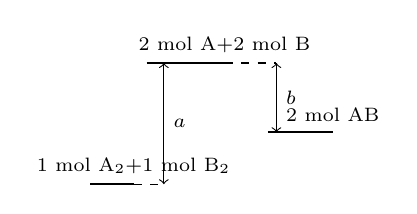
\begin{tikzpicture}[scale=0.55]
\axisEP{6.5}{4.4}
\draw[thick] (0.3,1)--(1.3,1) node[above]{\scriptsize 1 mol A$_2$+1 mol B$_2$};
\draw[thick] (1.6,3.8)--(3.4,3.8) node[above]{\scriptsize 2 mol A+2 mol B};
\draw[thick] (4.4,2.2)--(5.9,2.2) node[above]{\scriptsize 2 mol AB};
\draw[<->] (2,1)--(2,3.8) node[midway,right]{\scriptsize $a$};
\draw[<->] (4.6,2.2)--(4.6,3.8) node[midway,right]{\scriptsize $b$};
\draw[dashed] (1.3,1)--(2,1); \draw[dashed] (3.4,3.8)--(4.6,3.8);
\end{tikzpicture}
\end{center}
\xxb{每生成 2 mol AB(g) 吸收 $b$ kJ 热量}{$\Delta H=+(a-b)$ kJ·mol$^{-1}$}{反应物总能量高于生成物总能量}{断裂 1 mol A—A 和 1 mol B—B 放出 $a$ kJ 能量}

\item 已知 \ce{H2(g) + I2(g) <=> 2HI(g)} $\Delta H=-9.48$ kJ·mol$^{-1}$。下列说法正确的是\xz
\xxa{1 mol \ce{H2(g)} 与 1 mol \ce{I2(g)} 在密闭容器中充分反应，放出 9.48 kJ 热量}{生成 2 mol HI(g) 时放出 9.48 kJ 热量}{\ce{2HI(g) <=> H2(g) + I2(s)} 的 $\Delta H=+9.48$ kJ·mol$^{-1}$}{1 mol \ce{H2(g)} 与 1 mol \ce{I2(g)} 的总能量低于 2 mol HI(g) 的能量}
\end{xiti}

\zu{B组\quad 高考典型}
\begin{xiti}
\item \laiyuan{原创}\ \ce{CO2} 加氢制甲醇是实现“碳中和”的重要途径。已知：\\
①\ce{CO2(g) + H2(g) = CO(g) + H2O(g)} \quad $\Delta H_1=+41.2$ kJ·mol$^{-1}$\\
②\ce{CO(g) + 2H2(g) = CH3OH(g)} \quad $\Delta H_2=-90.7$ kJ·mol$^{-1}$\\
则 \ce{CO2(g) + 3H2(g) = CH3OH(g) + H2O(g)} 的 $\Delta H_3=$\tk kJ·mol$^{-1}$；该反应在\tk（填“高温”或“低温”）下更有利于自发进行（提示：$\Delta S<0$，可学完第3章再做）。

\item 下列各组热化学方程式中，$\Delta H_1>\Delta H_2$ 的是\xz
\xxa{\ce{C(s) + O2(g) = CO2(g)} $\Delta H_1$；\ce{C(s) + 1/2O2(g) = CO(g)} $\Delta H_2$}{\ce{S(s) + O2(g) = SO2(g)} $\Delta H_1$；\ce{S(g) + O2(g) = SO2(g)} $\Delta H_2$}{\ce{H2(g) + 1/2O2(g) = H2O(l)} $\Delta H_1$；\ce{H2(g) + 1/2O2(g) = H2O(g)} $\Delta H_2$}{\ce{CaO(s) + H2O(l) = Ca(OH)2(s)} $\Delta H_1$；\ce{CaCO3(s) = CaO(s) + CO2(g)} $\Delta H_2$}

\item 发射火箭可用液氢和液氧作推进剂。已知：①\ce{H2(g) + 1/2O2(g) = H2O(l)} $\Delta H_1=-285.8$ kJ·mol$^{-1}$；②\ce{H2(g) = H2(l)} $\Delta H_2=-0.92$ kJ·mol$^{-1}$；③\ce{O2(g) = O2(l)} $\Delta H_3=-6.84$ kJ·mol$^{-1}$；④\ce{H2O(l) = H2O(g)} $\Delta H_4=+44.0$ kJ·mol$^{-1}$。则 \ce{H2(l) + 1/2O2(l) = H2O(g)} 的 $\Delta H$ 为\xz
\xx{$+237.46$ kJ·mol$^{-1}$}{$-474.92$ kJ·mol$^{-1}$}{$-118.73$ kJ·mol$^{-1}$}{$-237.46$ kJ·mol$^{-1}$}

\item \laiyuan{2024年广东卷第19题(1)②，来源：仓库所附真题文档}\ 酸催化下 \ce{NaNO2} 与 \ce{NH4Cl} 混合溶液的反应（反应a）可用于石油开采中油路解堵。反应a：\ce{NO2^-(aq) + NH4^+(aq) = N2(g) + 2H2O(l)}。已知：\ce{NaNO2(s) + NH4Cl(s) = N2(g) + NaCl(s) + 2H2O(l)} $\Delta H_1$；\ce{NaNO2(s)} 溶解为 \ce{Na+(aq) + NO2^-(aq)} 的焓变为 $\Delta H_2$；\ce{NH4Cl(s)} 溶解为 \ce{Cl-(aq) + NH4^+(aq)} 的焓变为 $\Delta H_3$；\ce{NaCl(s)} 溶解为 \ce{Na+(aq) + Cl-(aq)} 的焓变为 $\Delta H_4$。则反应a的 $\Delta H=$\tk。

\item 已知石墨和金刚石的燃烧热 $\Delta H$ 分别为 $-393.5$ kJ·mol$^{-1}$、$-395.4$ kJ·mol$^{-1}$。下列说法正确的是\xz
\xxa{由石墨制备金刚石是放热过程}{等质量时，石墨的能量比金刚石的高}{石墨比金刚石稳定，石墨中 C—C 键的平均键能更大}{C（石墨，s）$=$ C（金刚石，s）$\Delta H=-1.9$ kJ·mol$^{-1}$}

\item \laiyuan{原创}\ 用 \ce{CH4} 催化还原 \ce{NO_x} 可消除氮氧化物污染。已知：①\ce{CH4(g) + 4NO2(g) = 4NO(g) + CO2(g) + 2H2O(g)} $\Delta H_1=-574$ kJ·mol$^{-1}$；②\ce{CH4(g) + 4NO(g) = 2N2(g) + CO2(g) + 2H2O(g)} $\Delta H_2=-1160$ kJ·mol$^{-1}$。(1) 写出 \ce{CH4} 将 \ce{NO2} 还原为 \ce{N2} 的热化学方程式（\ce{CH4} 的计量数为 1）。(2) 若用标准状况下 4.48 L \ce{CH4} 将 \ce{NO2} 还原为 \ce{N2}，放出的热量为多少？转移电子多少摩尔？

\item \laiyuan{原创}\ 已知键能（kJ·mol$^{-1}$）：\ce{N#N} 946，H—H 436，N—H 391。(1) 估算 \ce{N2(g) + 3H2(g) = 2NH3(g)} 的 $\Delta H$。(2) 从键能角度解释为什么 \ce{N2} 化学性质稳定，而合成氨反应却是放热反应。
\end{xiti}

\zu{C组\quad 冲刺高分}
\begin{xiti}
\item 白磷（\ce{P4}）、\ce{P4O6}、\ce{P4O10} 的分子结构：\ce{P4} 为正四面体，6 条棱为 P—P 键；\ce{P4O6} 是在 \ce{P4} 的每条 P—P 键中插入 1 个 O 原子；\ce{P4O10} 是在 \ce{P4O6} 基础上每个 P 原子再以 P=O 连接 1 个 O 原子。部分键能（kJ·mol$^{-1}$）：P—P 198，P—O 360，O=O 498，P=O $x$。
(1) 已知 1 mol 白磷完全燃烧生成 \ce{P4O10(s)} 的 $\Delta H=-2982$ kJ·mol$^{-1}$，求 $x$（忽略固态与气态的差别）。
(2) 0.5 mol 白磷与 \ce{O2} 反应完全生成 \ce{P4O6} 放出多少热量？
(3) 已知 \ce{P4}（白磷，s）$=$ 4P（红磷，s）$\Delta H=-29.2$ kJ·mol$^{-1}$，判断白磷、红磷哪种更稳定，并比较二者燃烧热的大小。

\item \laiyuan{原创}\ 甲烷干重整（\ce{CH4 + CO2 -> 2CO + 2H2}）可同时利用两种温室气体。已知 25 ℃ 时 \ce{CH4(g)}、\ce{CO(g)}、\ce{H2(g)} 的燃烧热 $\Delta H$ 分别为 $-890.3$、$-283.0$、$-285.8$ kJ·mol$^{-1}$；\ce{H2O(l) = H2O(g)} $\Delta H=+44.0$ kJ·mol$^{-1}$。
(1) 求 \ce{CH4(g) + CO2(g) = 2CO(g) + 2H2(g)} 的 $\Delta H$。
(2) 若将产物中的 \ce{H2} 全部燃烧生成水蒸气，求 \ce{2H2(g) + O2(g) = 2H2O(g)} 的 $\Delta H$。
(3) 有人认为“干重整是吸热反应，所以没有利用价值”。结合 (1)(2) 及能量守恒，评价该观点。

\item \laiyuan{原创}\ \ce{CO2} 加氢制甲醇可经两条途径：途径Ⅰ直接反应 \ce{CO2(g) + 3H2(g) = CH3OH(g) + H2O(g)} $\Delta H_1$；途径Ⅱ先发生 \ce{CO2(g) + H2(g) = CO(g) + H2O(g)} $\Delta H_2=+41.2$ kJ·mol$^{-1}$，再发生 \ce{CO(g) + 2H2(g) = CH3OH(g)} $\Delta H_3=-90.7$ kJ·mol$^{-1}$。已知 \ce{H2O(l) = H2O(g)} $\Delta H=+44.0$ kJ·mol$^{-1}$。(1) 求 $\Delta H_1$。(2) 求 \ce{CO2(g) + 3H2(g) = CH3OH(g) + H2O(l)} 的 $\Delta H$。(3) 画出途径Ⅱ的能量示意图（标出中间状态），并判断哪一步需要从外界获得能量。(4) 若在途径Ⅱ中加入只加快第二步的催化剂，总反应的 $\Delta H$ 是否改变？
\end{xiti}

% ------------------------------------------------------------
\zhangmo{练习解析}
\begin{jiexilist}
\item \ans{B}A 错：吸热反应不一定需加热，如 \ce{Ba(OH)2*8H2O} 与 \ce{NH4Cl}。B 对：反应物总能量高，多余能量放出，$\Delta H<0$。C 错：溶解是物理过程，不是“放热反应”。D 错：$\Delta H$ 只与始终态有关，与条件无关。
\item \ans{C}A 错：温度计不能搅拌，易损坏且测温不准。B 错：生成 \ce{BaSO4} 沉淀也放热，测得值偏大，不能用于测定中和反应反应热。C 对：反应放热使温度升高，最高温度对应反应恰好完成、散热最少的时刻。D 错：醋酸电离吸热，测得放热数值偏小。
\item \ans{B}1 g \ce{H2} 为 0.5 mol，故 1 mol \ce{H2} 生成液态水放热 285.8 kJ。A 中 2 mol \ce{H2} 应为 $-571.6$；C 未标状态；D 中生成的是 \ce{H2O(g)}，放热应少于 285.8 kJ。
\item \ans{C}A 错：碳的指定产物是 \ce{CO2(g)}。B 错：H 元素的指定产物是 \ce{H2O(l)}。C 对：燃烧热用 $\Delta H$ 表示时带负号。D 错：燃烧热以 1 mol 可燃物为标准，是定值；放出的总热量才与物质的量成正比。
\item \ans{$-482$ kJ·mol$^{-1}$；$-285$ kJ·mol$^{-1}$}$\Delta H=2\times436+498-4\times463=872+498-1852=-482$ kJ·mol$^{-1}$（1 个 \ce{H2O} 含 2 个 H—O）。生成 1 mol \ce{H2O(g)}：$-241$ kJ·mol$^{-1}$；再液化放热 44 kJ：$-241-44=-285$ kJ·mol$^{-1}$。
\item \ans{B}由图：断开 1 mol \ce{A2} 和 1 mol \ce{B2} 生成气态原子吸收 $a$ kJ，原子形成 2 mol AB 放出 $b$ kJ，且 $a>b$（2 mol AB 能量高于反应物），故 $\Delta H=+(a-b)$ kJ·mol$^{-1}$，反应吸热，A、C 错；断键吸热，D 错。
\item \ans{B}A：可逆反应不能进行完全，放热小于 9.48 kJ；B：$\Delta H$ 对应按方程式完全生成 2 mol HI(g)，正确；C：生成物为 \ce{I2(s)}，与 \ce{I2(g)} 能量不同，$\Delta H$ 不等于 $+9.48$；D：放热反应，反应物总能量高于生成物。
\item \ans{$-49.5$；低温}①$+$②得目标式，$\Delta H_3=41.2-90.7=-49.5$ kJ·mol$^{-1}$。$\Delta H<0$、$\Delta S<0$，由 $\Delta G=\Delta H-T\Delta S<0$ 可知低温有利于自发。
\item \ans{B}A：完全燃烧放热多，$\Delta H_1<\Delta H_2$。B：S(g) 能量高于 S(s)，燃烧放热更多，$\Delta H_2<\Delta H_1$，即 $\Delta H_1>\Delta H_2$，符合题意。C：生成液态水多放出液化热，$\Delta H_1<\Delta H_2$。D：\ce{CaO} 与水化合放热 $\Delta H_1<0$，\ce{CaCO3} 分解吸热 $\Delta H_2>0$，$\Delta H_1<\Delta H_2$。
\item \ans{D}目标式$=$①$-$②$-\frac12$③$+$④：\ce{H2(l)} 只在②中且需在反应物侧，故 $-$②；\ce{O2(l)} 只在③中，取 $-\frac12$③；\ce{H2O(g)} 只在④中，取 $+$④。$\Delta H=-285.8+0.92+\frac12\times6.84+44.0=-237.46$ kJ·mol$^{-1}$。
\item \ans{$\Delta H_1-\Delta H_2-\Delta H_3+\Delta H_4$}设计途径：\ce{NO2^-(aq) + NH4^+(aq)}（与 \ce{Na+}、\ce{Cl-} 一起）$\xrightarrow{-\Delta H_2-\Delta H_3}$ \ce{NaNO2(s) + NH4Cl(s)} $\xrightarrow{\Delta H_1}$ \ce{N2(g) + NaCl(s) + 2H2O(l)} $\xrightarrow{\Delta H_4}$ \ce{N2(g) + Na+(aq) + Cl-(aq) + 2H2O(l)}。\ce{Na+}、\ce{Cl-} 为旁观离子，两端相同，故反应a的 $\Delta H=\Delta H_1-\Delta H_2-\Delta H_3+\Delta H_4$。
\item \ans{C}由燃烧热求得 C（石墨）$\to$ C（金刚石）$\Delta H=-393.5-(-395.4)=+1.9$ kJ·mol$^{-1}$，吸热，A、D 错；石墨能量低、更稳定，B 错；石墨更稳定，其中化学键更牢固，C 对。
\item (1) (①$+$②)$\div2$：\ce{CH4(g) + 2NO2(g) = N2(g) + CO2(g) + 2H2O(g)} $\Delta H=\frac{-574-1160}{2}=-867$ kJ·mol$^{-1}$。(2) $n(\ce{CH4})=0.2$ mol，放热 $0.2\times867=173.4$ kJ；C 由 $-4\to+4$，每个 \ce{CH4} 失 8 个电子，转移 1.6 mol 电子。
\item (1) $\Delta H=946+3\times436-6\times391=-92$ kJ·mol$^{-1}$。(2) \ce{N#N} 键能很大，断开它需要很高的能量（活化能大），所以 \ce{N2} 很稳定、常温难反应；但生成物中 6 个 N—H 键放出的能量（2346 kJ）大于断开 1 个 \ce{N#N} 和 3 个 H—H 吸收的能量（2254 kJ），所以总反应放热。“稳定”说的是反应难易（与活化能有关），“放热”说的是能量高低，两者不矛盾。
\item \textbf{(1)} $x=585$。\ce{P4 + 5O2 = P4O10}：断键 $6\times198+5\times498=3678$ kJ；\ce{P4O10} 含 12 个 P—O 和 4 个 P=O，成键 $12\times360+4x$。$3678-(4320+4x)=-2982$，解得 $x=585$。
\textbf{(2)} 819 kJ。\ce{P4 + 3O2 = P4O6}：$\Delta H=6\times198+3\times498-12\times360=-1638$ kJ·mol$^{-1}$；0.5 mol 放热 819 kJ。
\textbf{(3)} 白磷转化为红磷放热，红磷能量低，红磷更稳定；等质量（同为 4 mol P）燃烧时，白磷放热更多，白磷的燃烧热（以 \ce{P4} 计）比 4 mol 红磷燃烧放出的热量多 29.2 kJ，即单位质量白磷燃烧放热更多。
\item \textbf{(1)} $\Delta H=+247.3$ kJ·mol$^{-1}$。燃烧热法：$\Delta H=\Delta_\text{c}H(\ce{CH4})+\Delta_\text{c}H(\ce{CO2})-2\Delta_\text{c}H(\ce{CO})-2\Delta_\text{c}H(\ce{H2})=-890.3+0+566.0+571.6=+247.3$ kJ·mol$^{-1}$（\ce{CO2} 是最终产物，燃烧热为 0）。
\textbf{(2)} \ce{2H2(g) + O2(g) = 2H2O(l)} $\Delta H=-571.6$ kJ·mol$^{-1}$，再加 \ce{2H2O(l) = 2H2O(g)} $+88.0$，得 $\Delta H=-483.6$ kJ·mol$^{-1}$。
\textbf{(3)} 观点片面。干重整吸收的能量（247.3 kJ）储存在产物 CO 和 \ce{H2} 中，产物燃烧时可以释放出来：1 mol \ce{CH4} 直接燃烧放热 890.3 kJ，而干重整产物 2 mol CO 和 2 mol \ce{H2} 燃烧（生成液态水）放热 $566.0+571.6=1137.6$ kJ，恰好比 890.3 kJ 多 247.3 kJ（能量守恒）。若用太阳能、工业余热等廉价能量驱动干重整，就能把低品位热能转化为化学能储存，同时消耗 \ce{CO2}、得到合成气（CO、\ce{H2}，化工原料），具有利用价值。
\item (1) $\Delta H_1=\Delta H_2+\Delta H_3=41.2-90.7=-49.5$ kJ·mol$^{-1}$。(2) 再加上 \ce{H2O(g) = H2O(l)}（$-44.0$）：$-49.5-44.0=-93.5$ kJ·mol$^{-1}$。(3) 示意图：起点“\ce{CO2(g) + 3H2(g)}”，第一步升高 41.2 kJ 到“\ce{CO(g) + H2O(g) + 2H2(g)}”，第二步降低 90.7 kJ 到终点“\ce{CH3OH(g) + H2O(g)}”，终点比起点低 49.5 kJ；第一步吸热，需要从外界获得能量。(4) 不改变，$\Delta H$ 只与始终态有关。
\end{jiexilist}
